
%(BEGIN_QUESTION)
% Copyright 2006, Tony R. Kuphaldt, released under the Creative Commons Attribution License (v 1.0)
% This means you may do almost anything with this work of mine, so long as you give me proper credit

Choose proper resistor values so that the op-amp outputs a 0 to 5 volt voltage signal over a temperature measurement range of 0$^{o}$ C to 80$^{o}$ C.  Assume the use of a 1000 $\Omega$ RTD with a European alpha.

$$\includegraphics[width=15.5cm]{i00411x01.eps}$$

\vskip 20pt \vbox{\hrule \hbox{\strut \vrule{} {\bf Suggestions for Socratic discussion} \vrule} \hrule}

\begin{itemize}
\item{} Do the operational amplifier's two feedback resistors affect this temperature circuit's {\it zero}, {\it span}, or {\it linearity}?
\item{} How might we provide for {\it adjustable} zero and span calibrations in this circuit?
\item{} Choose a resistor at random in this circuit and imagine that it fails (either open or shorted).  Would this electrical fault make the RTD appear hotter than it really is, or colder than it really is?  Explain your answer in detail.
\end{itemize}

\underbar{file i00411}
%(END_QUESTION)





%(BEGIN_ANSWER)

At 0 degrees C, $R_{RTD}$ = 1000 $\Omega$ and $V_{+}$ = 0 volts

\vskip 10pt

At 80 degrees C, $R_{RTD}$ = 1308 $\Omega$ and $V_{+}$ = 0.06672 volts (assuming all other resistors in the bridge are 1k $\Omega$ each)

\vskip 10pt

In order to achieve a 5 volt opamp output given a 66.72 mV input, we need a voltage gain of exactly 74.935.  Given the fact that this opamp circuit is noninverting, and its voltage gain is the ratio of feedback resistors plus one, we need a resistor ratio of 73.935:1.

\vskip 10pt

The following resistor values are suggested, but are not the {\it only} correct values that may be used to obtain the same calibration:

$$\includegraphics[width=15.5cm]{i00411x02.eps}$$

%(END_ANSWER)





%(BEGIN_NOTES)









\vskip 20pt \vbox{\hrule \hbox{\strut \vrule{} {\bf Virtual Troubleshooting} \vrule} \hrule}

This question is a good candidate for a ``Virtual Troubleshooting'' exercise.  Presenting the diagram to students, you first imagine in your own mind a particular fault in the system.  Then, you present one or more symptoms of that fault (something noticeable by an operator or other user of the system).  Students then propose various diagnostic tests to perform on this system to identify the nature and location of the fault, as though they were technicians trying to troubleshoot the problem.  Your job is to tell them what the result(s) would be for each of the proposed diagnostic tests, documenting those results where all the students can see.

During and after the exercise, it is good to ask students follow-up questions such as:

\begin{itemize}
\item{} What does the result of the last diagnostic test tell you about the fault?
\item{} Suppose the results of the last diagnostic test were different.  What then would that result tell you about the fault?
\item{} Is the last diagnostic test the best one we could do?
\item{} What would be the ideal order of tests, to diagnose the problem in as few steps as possible?
\end{itemize}


%INDEX% Measurement, temperature: RTD

%(END_NOTES)


